\documentclass[11pt]{amsart}
\usepackage{geometry}                % See geometry.pdf to learn the layout options. There are lots.
\geometry{letterpaper}                   % ... or a4paper or a5paper or ... 
%\geometry{landscape}                % Activate for for rotated page geometry
\usepackage[parfill]{parskip}    % Activate to begin paragraphs with an empty line rather than an indent
\usepackage{graphicx}
\usepackage{amssymb}
\usepackage{epstopdf}  
\usepackage{hyperref}
  \usepackage{color}
  \definecolor{linkcol}{rgb}{0,0,0.4}
  \definecolor{citecol}{rgb}{0.5,0,0}
  \hypersetup
  {
  pdfauthor="Mathieu Guigue", %auteur du document
  %pdftoolbar=false, %barre d'outils non visible 
  pdfmenubar=true, %barre de menu visible
  colorlinks=true, %couleurs sur les liens hypertextes
  pdfpagemode=UseNone, %aucun mode de page
  pdfpagelayout=SinglePage, %ouverture en simple page
  pdffitwindow=true, %pages ouvertes entierement dans toute la fenetre
  linkcolor=linkcol, %couleur des liens hypertextes internes
  citecolor=citecol, %couleur des liens pour les citations
  urlcolor=linkcol %couleur des liens pour les url
  }
\DeclareGraphicsRule{.tif}{png}{.png}{`convert #1 `dirname #1`/`basename #1 .tif`.png}

\newtheorem{tgf}{To-Go-Further}


\title{Report about the assignment}
\author{Mathieu Guigue}
\date{\today}                                           % Activate to display a given date or no date

\begin{document}
\maketitle

\section{Introduction}

Meteorological data such as the atmospherical pressure, the relative humidity and the temperature have been provided over several days.
The goal of this study is to extract relationships between these variables.

NetCDF4 files containing the data collected over a day have been given.
The first part of the assignment consists in reducing the amount of data and especially removing the statistical fluctuations in the data that don't bing any useful piece of informations.
A second part aims at finding clusters in the parameters space corresponding to locations where the parameters share similar behaviors.

\section{Part 1: Data averaging}
\subsection{Time series}

Figure \ref{fig:ts-data} shows the data time series as extracted from the files.
\begin{figure}
    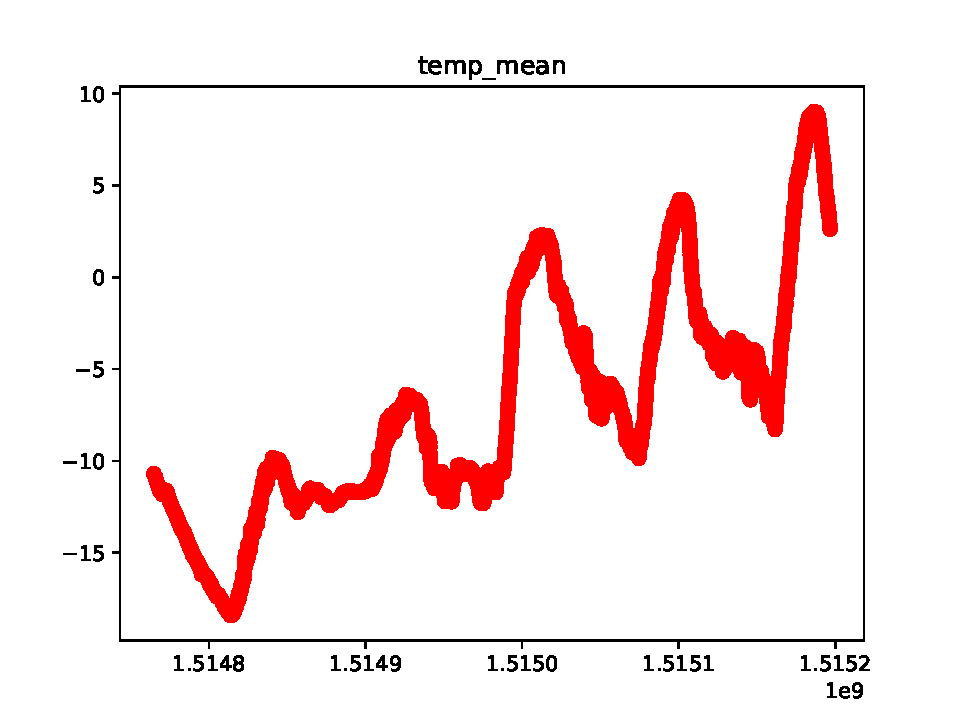
\includegraphics[width=0.45\textwidth]{../plots/temp_mean.pdf}
    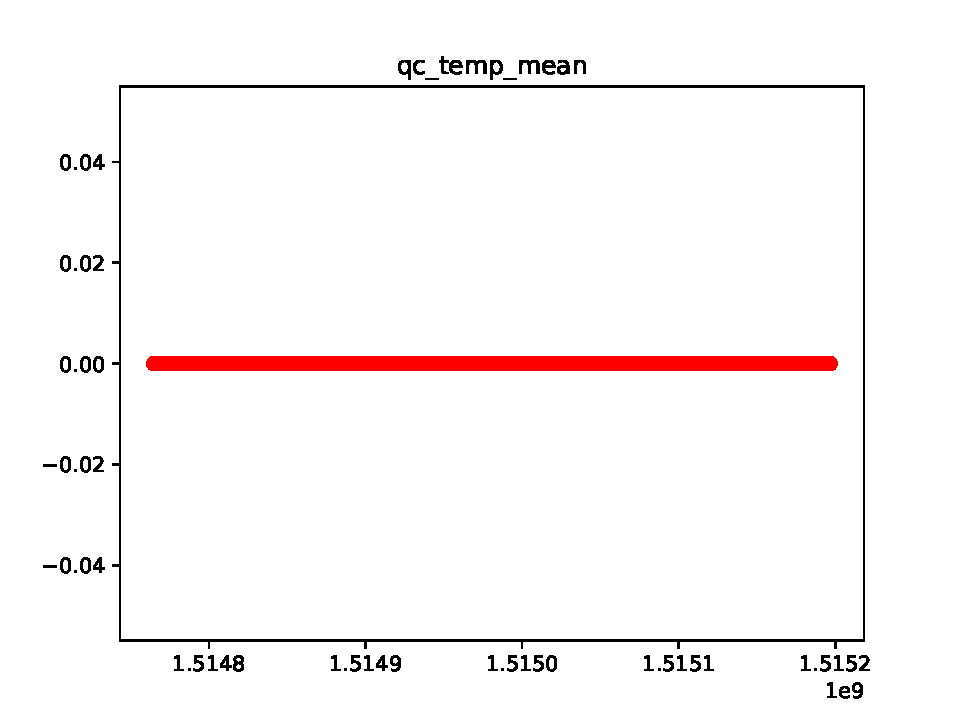
\includegraphics[width=0.45\textwidth]{../plots/qc_temp_mean.pdf}
    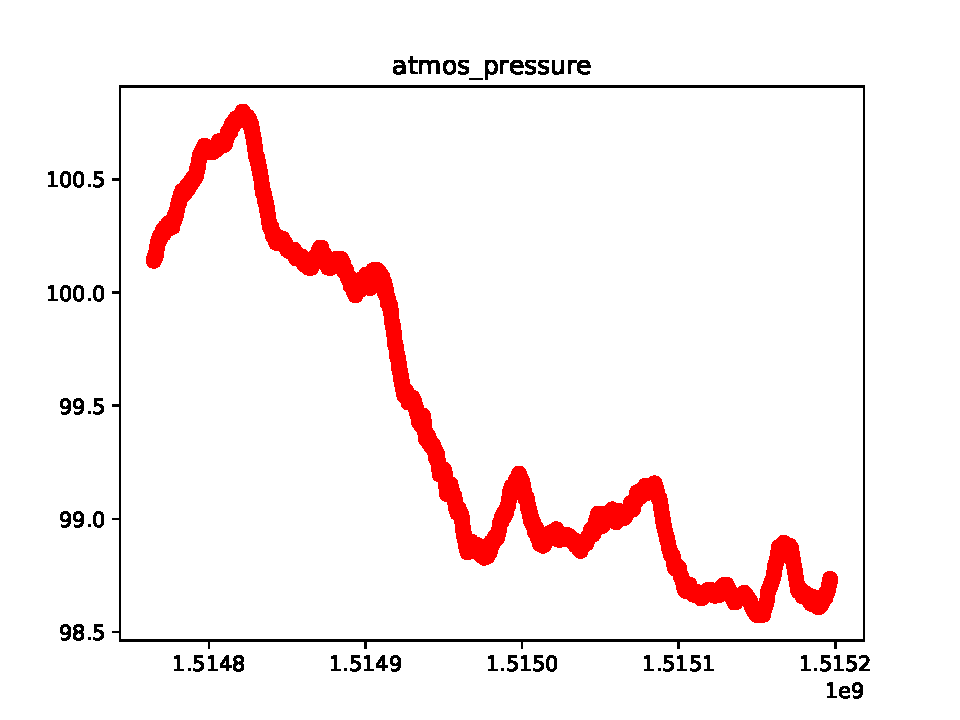
\includegraphics[width=0.45\textwidth]{../plots/atmos_pressure.pdf}
    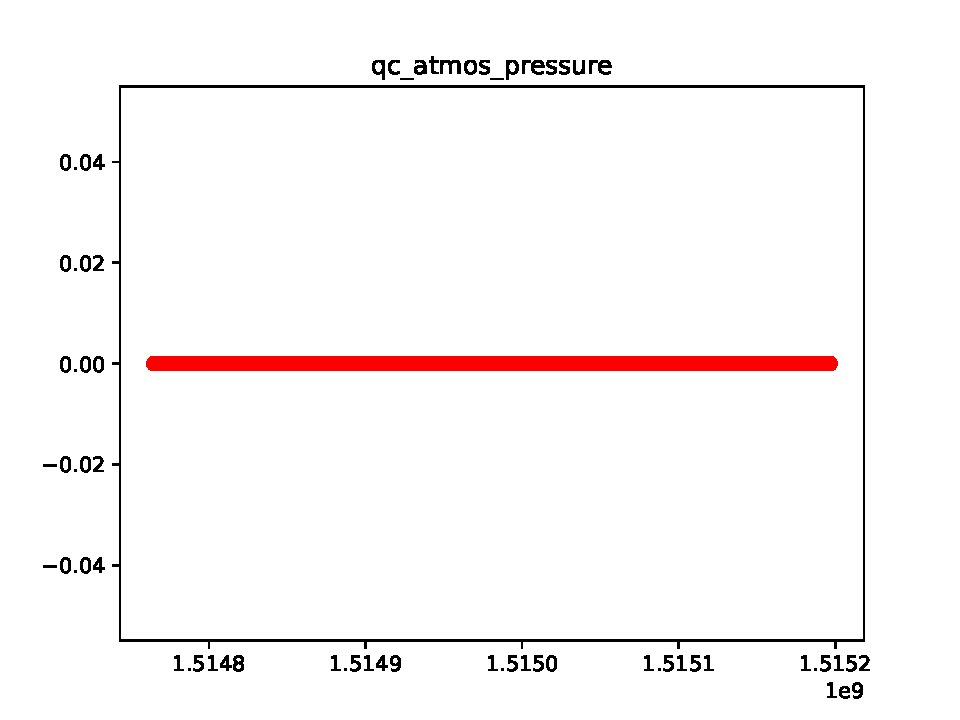
\includegraphics[width=0.45\textwidth]{../plots/qc_atmos_pressure.pdf}
    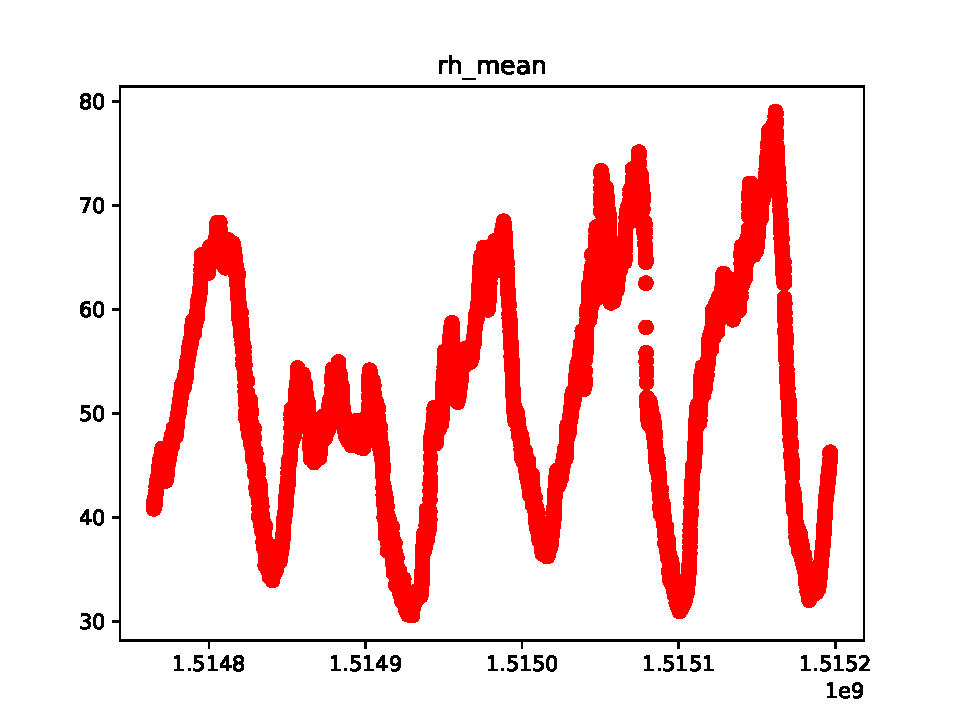
\includegraphics[width=0.45\textwidth]{../plots/rh_mean.pdf}
    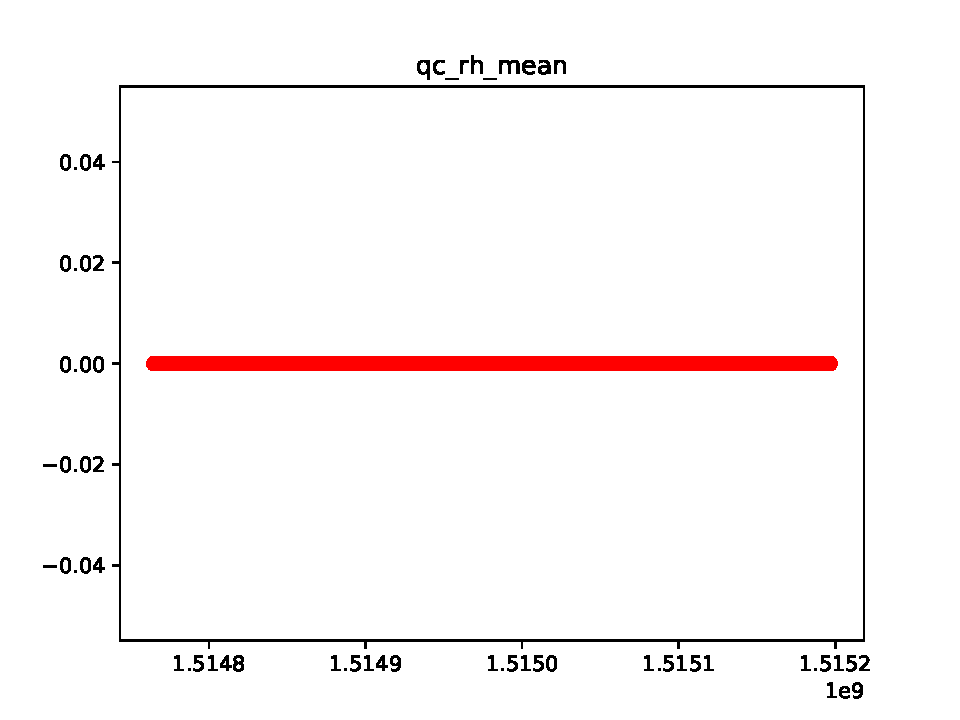
\includegraphics[width=0.45\textwidth]{../plots/qc_rh_mean.pdf}
    \caption{\label{fig:ts-data}Time series of the mean temperature, mean relative humidity and atmospheric pressure (left) and the associated quality check value (right) as a function of time.}
\end{figure}
We have 5 days of data, with datapoints each 60 seconds.
We verify that the data quality checks are good for all of these data.
%\begin{figure}
%    \caption{Time series of the quality checks for mean temperature, mean relative humidity and atmospheric pressure as a function of time.}
%\end{figure}

Each file corresponds to a day of data, one data point every 60 seconds.
Each day has its own time stamp (number of seconds since midnight) and a hardcoded-modification of the reader function is required to get things working.

\subsection{Estimating the optimal average period}

In the assignment a data averaging over 5 minutes (5 points) is requested.
This aims at reducing the measurements fluctuations which are not bringing informations to the analysis (a.k.a. white noise fluctuations).

We can try to estimate the optimal value for such averaging.
Using an Allan\footnote{\href{https://en.wikipedia.org/wiki/Allan_variance}{Allan Variance wiki page}} representation of the data, I can estimate what the typical period where the measurements fluctuations are Gaussian is.
Figure \ref{fig:asd} shows the Allan Standard Deviation as a function of the averaging period.
\begin{figure}
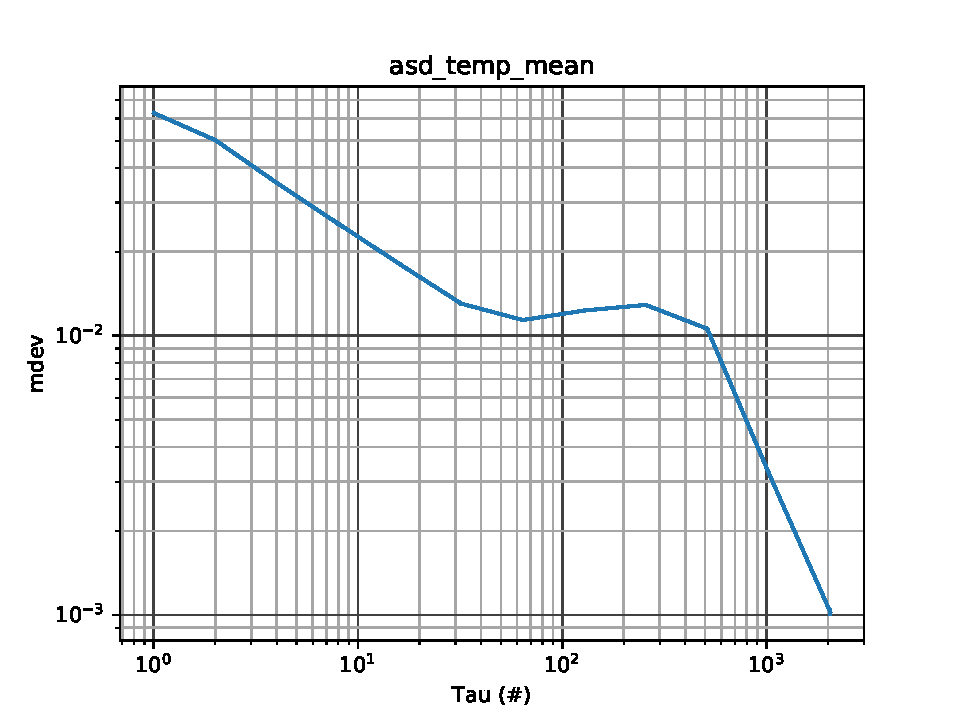
\includegraphics[width=0.45\textwidth]{../plots/asd_temp_mean.pdf}
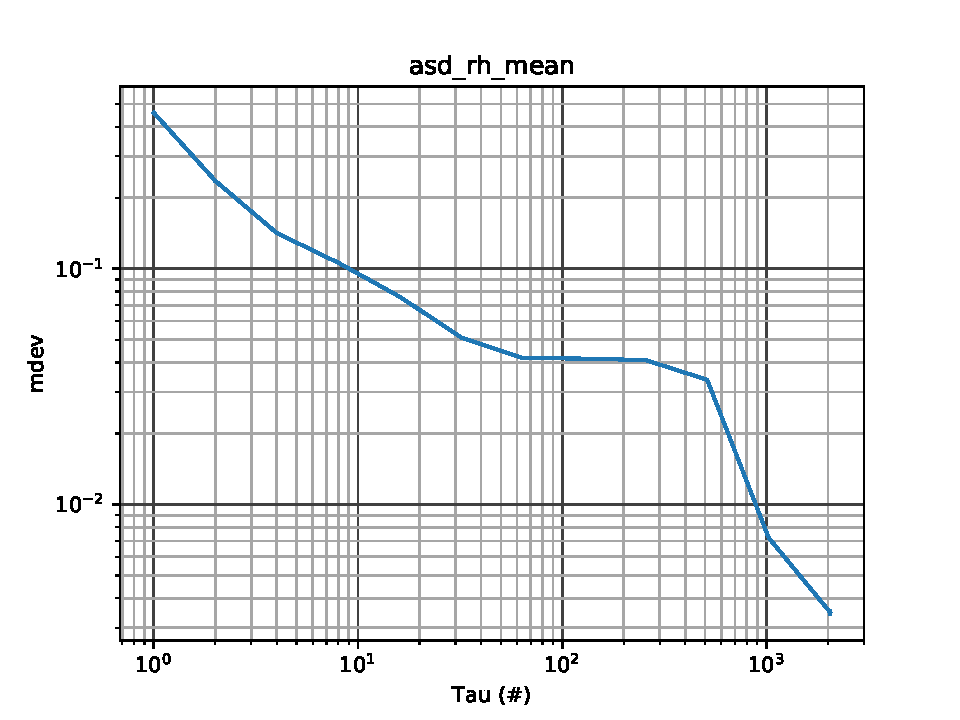
\includegraphics[width=0.45\textwidth]{../plots/asd_rh_mean.pdf}
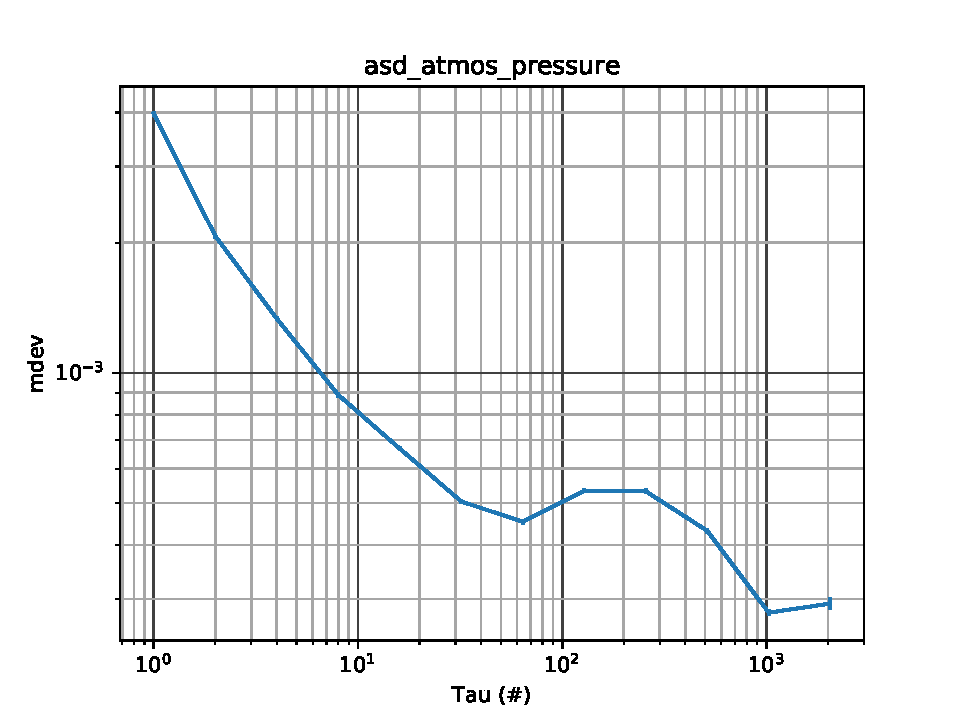
\includegraphics[width=0.45\textwidth]{../plots/asd_atmos_pressure.pdf}
\caption{\label{fig:asd}Allan Standard Deviation of the mean temperature, mean relative humidity and atmospheric pressure as a function of the period (in number of samples).}
\end{figure}
For short averaging period, the deviation decreases as the fluctuations are purely white.
At some point, the deviation stops decreasing: this can be interpreted as this is the typical moment at which fluctuations are not Gaussian anymore.
The corresponding averaging period would then be the optimal averaging period.
It seems that the value at which non Gaussian fluctuations appear is defined for all three variables to be about 50 samples.
{\tgf Implement an algorithmic way to extract from the Allan Standard Deviation the number of measurements to average (something like a minimum finder).}

The averaged data (represented on Figure \ref{fig:ts-avg}) are then saved in a CDF file named sgpmetavgE13.b1.20180101.000000.cdf.
\begin{figure}
    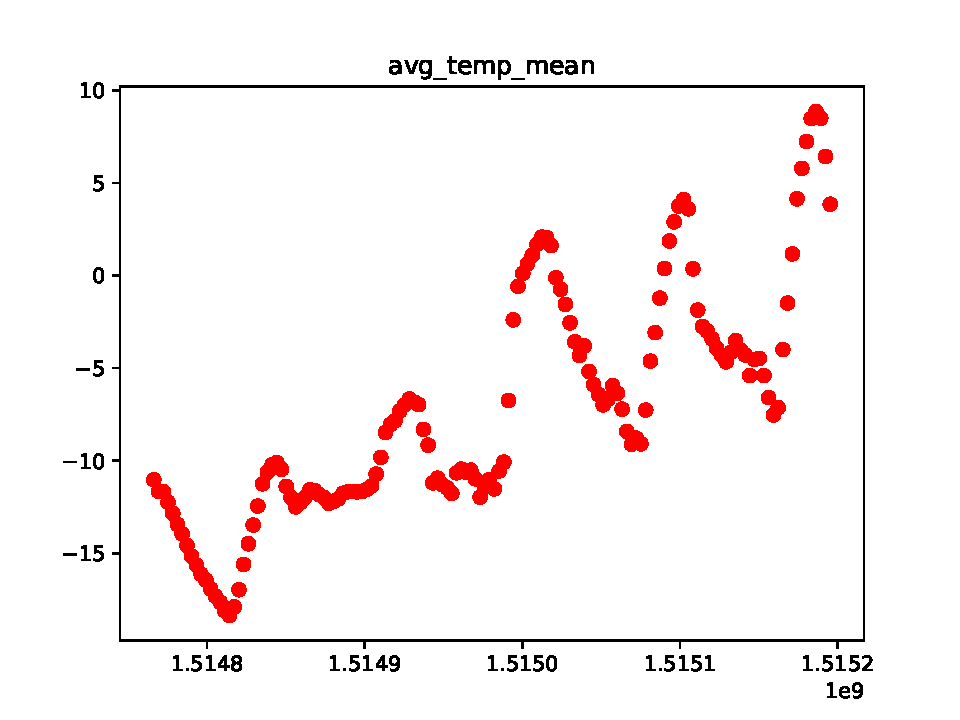
\includegraphics[width=0.45\textwidth]{../plots/avg_temp_mean.pdf}
    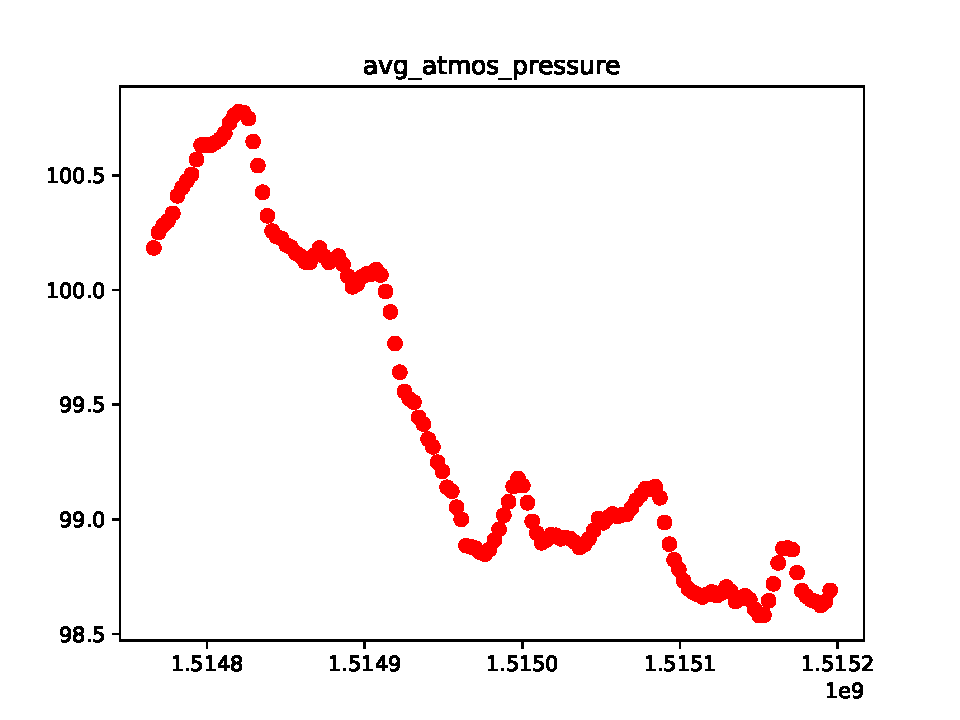
\includegraphics[width=0.45\textwidth]{../plots/avg_atmos_pressure.pdf}
    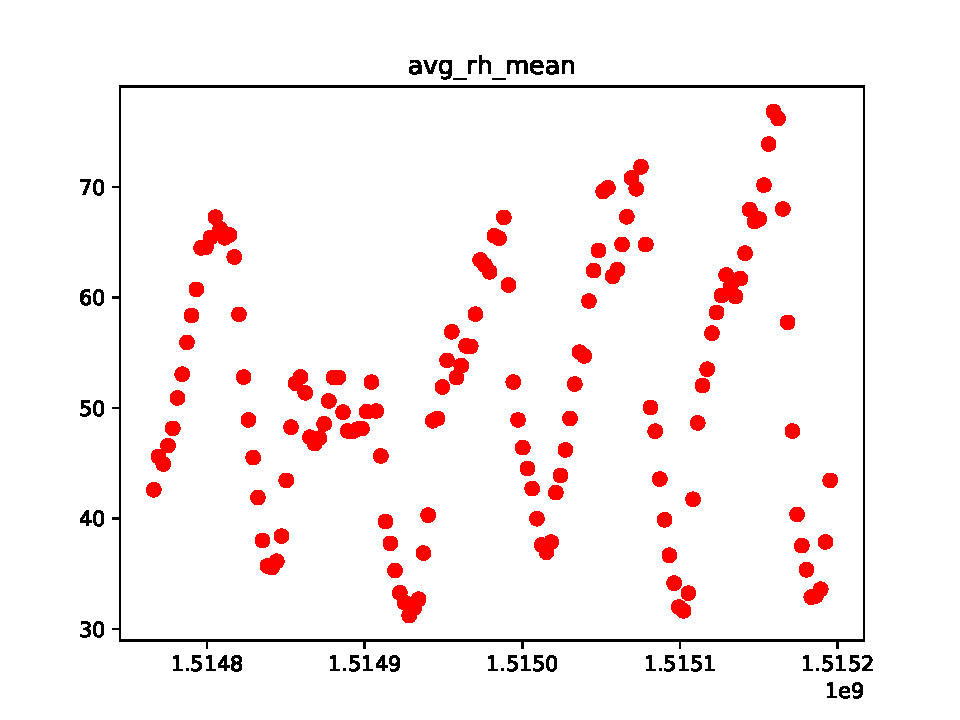
\includegraphics[width=0.45\textwidth]{../plots/avg_rh_mean.pdf}
    \caption{\label{fig:ts-avg}Time series of the average of mean temperature, mean relative humidity and atmospheric pressure as a function of time.}
\end{figure}

\section{Part 2: Clustering of data}

\subsection{$k$-means algorithm}
The goal here is to determine how the data are clustered.
The features we will use to find these clusters are the average temperature, atmospheric pressure and relative humidity and the derivatives of these quantities.
The clusters locations are determined using a $k$-means clustering algorithm that works in 2 steps that are repeated until convergence.
Given a number of cluster to find and a initial guess of the clusters centers, it first assigns all the data points to a cluster by determining the closest cluster center to each datapoint.
Then it calculates the average position of the obtained cluster.

Here I have used the Scipy clustering package\footnote{\href{https://docs.scipy.org/doc/scipy/reference/cluster.vq.html}{Scipy clustering package}}.
Figure \ref{fig:distance_to_centroids} shows the distance between the datapoints and each cluster center for various numbers of clusters. 
\begin{figure}
    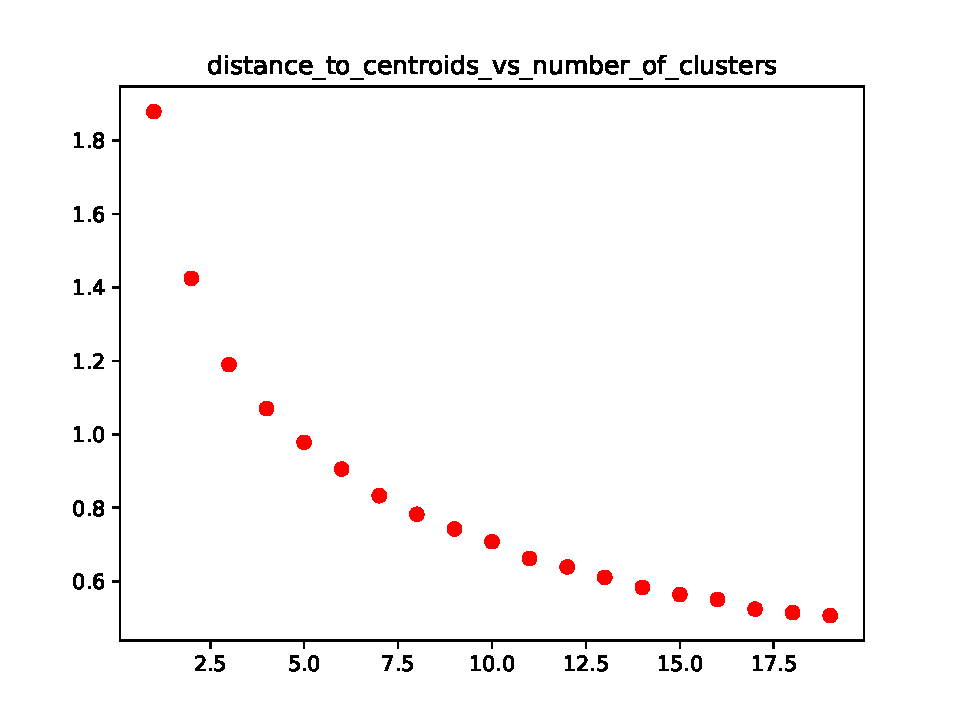
\includegraphics[width=0.45\textwidth]{../plots/distance_to_centroids_vs_number_of_clusters.pdf}
    \caption{\label{fig:distance_to_centroids} Distance to the cluster centers as a function of the number of clusters for the entire dataset.}
\end{figure}

\subsection{Determination of the optimal number of clusters} 

If the number of clusters we assume exists is too large, we encounter a over-fitting (or over-interpretation) issue, where statistical fluctuations are interpreted as characteristics that actually don't exist.
The optimization of the number of clusters consists in determining the transition location when overfitting happens.

The derivative of the average temperature is calculated and used in this study.
We divide the dataset in two subsets: 90 \% goes as training dataset and the rest as testing set.
A shuffling of the data is done, so the time correlations can be ignored.
We then determine the clusters locations using the training set and we estimate the distance between the testing set data and the clusters centers.
For several numbers of clusters, we repeat this procedure and extract the average distance.
Figure \ref{fig:distance_to_centroids2} shows the results of this approach.
\begin{figure}
    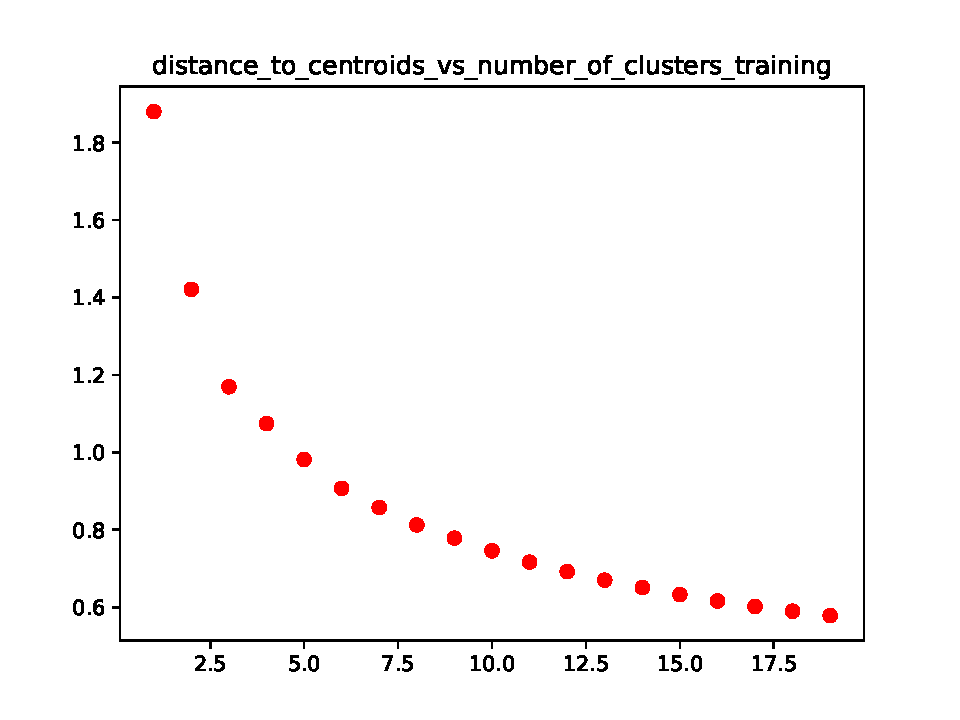
\includegraphics[width=0.45\textwidth]{../plots/distance_to_centroids_vs_number_of_clusters_training_5.pdf}
    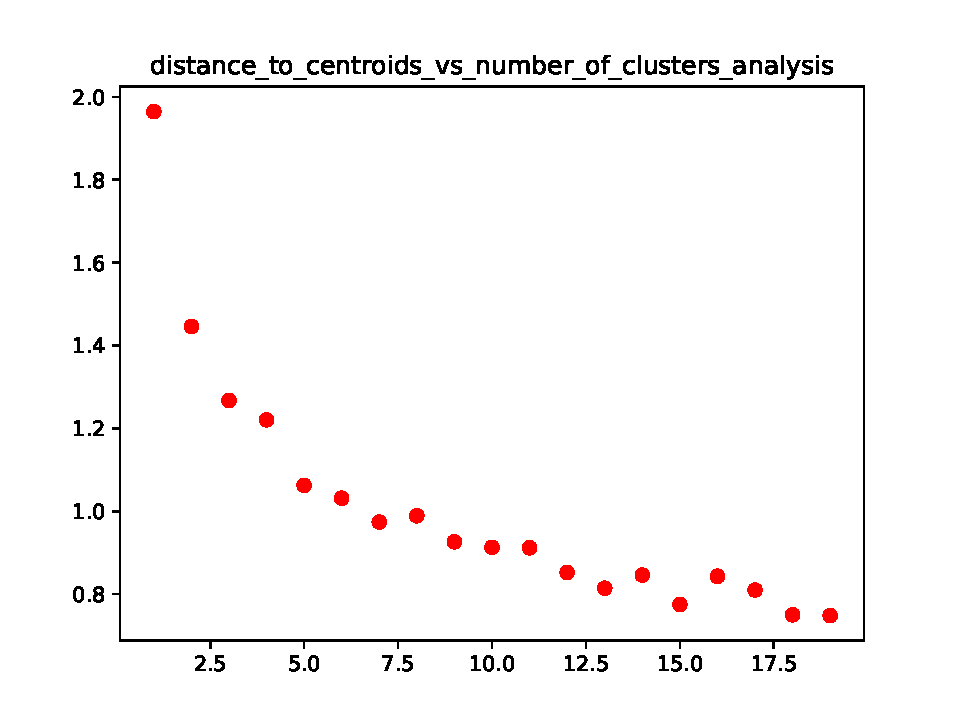
\includegraphics[width=0.45\textwidth]{../plots/distance_to_centroids_vs_number_of_clusters_analysis_5.pdf}
    \caption{\label{fig:distance_to_centroids2} Distance to the cluster centers as a function of the number of clusters for a 5 minutes averaging: the plot on the right corresponds to the training dataset and the right to the testing dataset.}
\end{figure}
We can see that, as we can expect, the more cluster the better the algorithm is performing on the training set.
A similar behavior is observed for the testing data, but the distances are generally larger for this set.

The best value for the number of clusters could be when the improvement rate of the algorithm in classifying the data decreases because it starts to explain statistical fluctuations by using clusters.
On the figure \ref{fig:distance_to_centroids2}, this corresponds to a change in the slope of the distance to centroids.
On the training set, this phenomenon appears around $k=6$.
A similar inflection point appears for the testing set around $k=6$.
The optimal number of clusters seems to be about 6.

As a comparison, the figure \ref{fig:distance_to_centroids3} shows the distance to the cluster centers as a function of the number of cluster, but for an averaging of the data of 50 minutes (instead of 5, as requested by the assignment).
The same conclusions can be drawn.
However a difference in the absolute values of these distances is observed, this would required some investigations to understand what is causing this.
\begin{figure}
    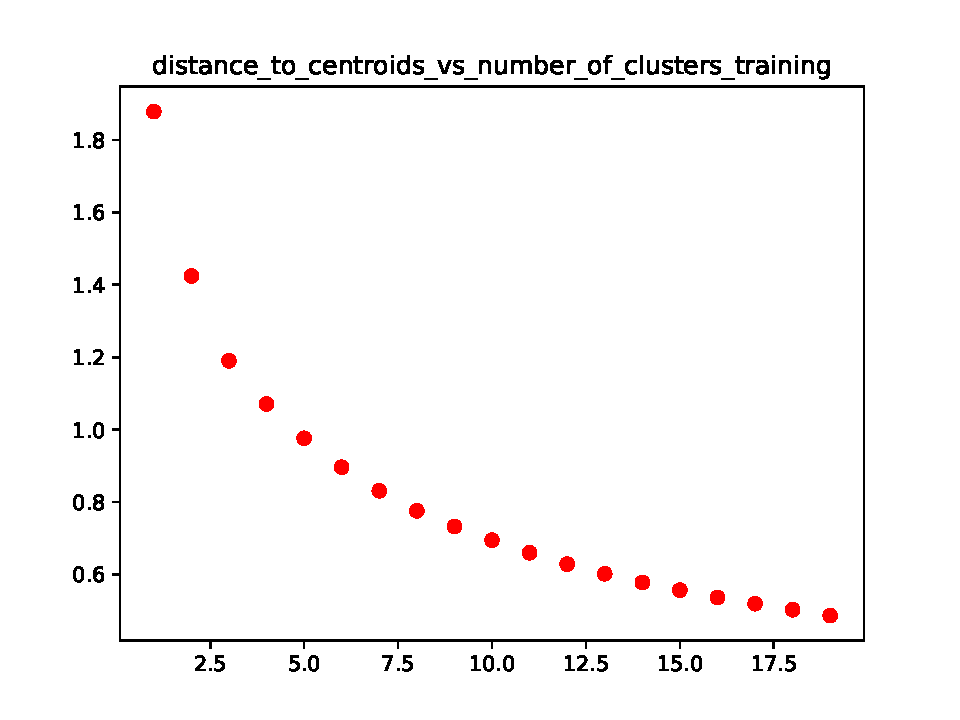
\includegraphics[width=0.45\textwidth]{../plots/distance_to_centroids_vs_number_of_clusters_training.pdf}
    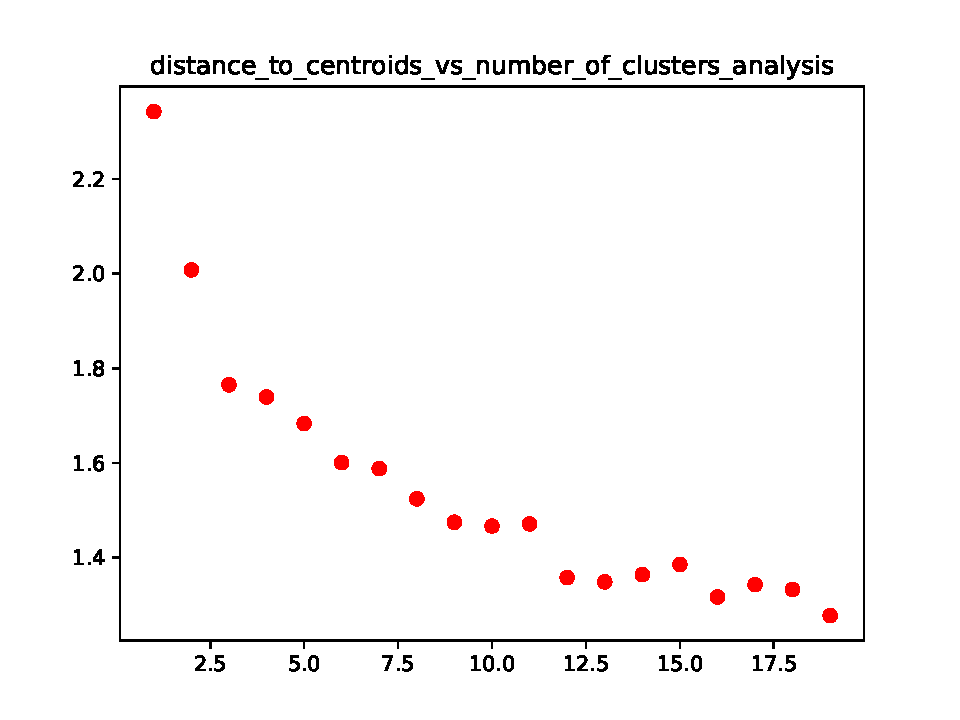
\includegraphics[width=0.45\textwidth]{../plots/distance_to_centroids_vs_number_of_clusters_analysis.pdf}
    \caption{\label{fig:distance_to_centroids3} Distance to the cluster centers as a function of the number of clusters for a 50 minutes averaging: the plot on the right corresponds to the training dataset and the right to the testing dataset.}
\end{figure}

Figure \ref{fig:2dplots} shows the 2D representations of the data with the centroids location using $k=6$.
\begin{figure}
    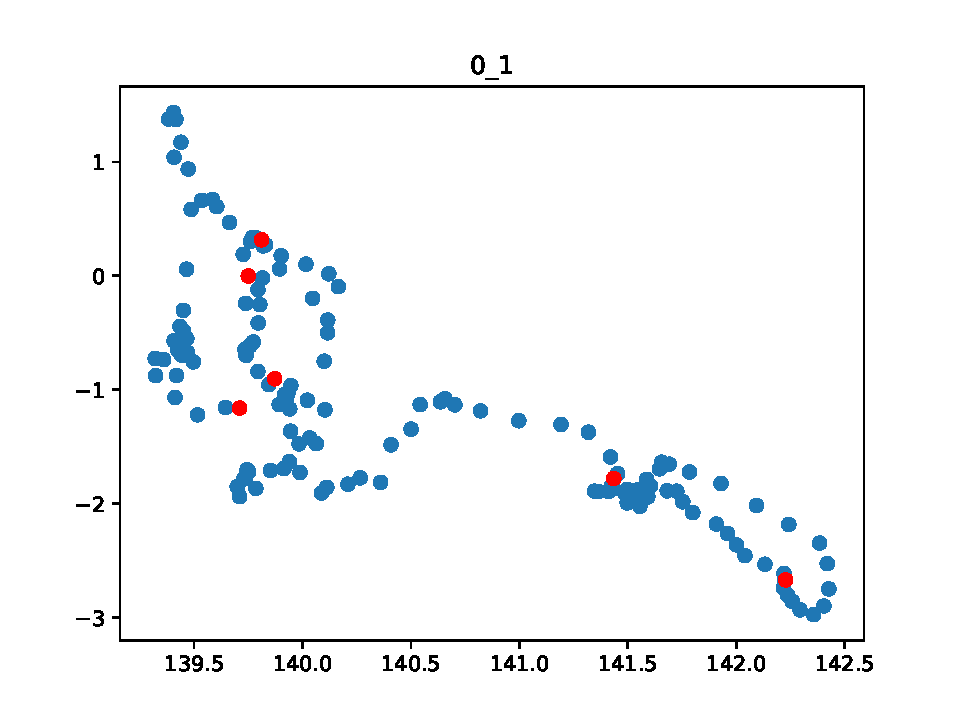
\includegraphics[width=0.45\textwidth]{../plots/0_1.pdf}
    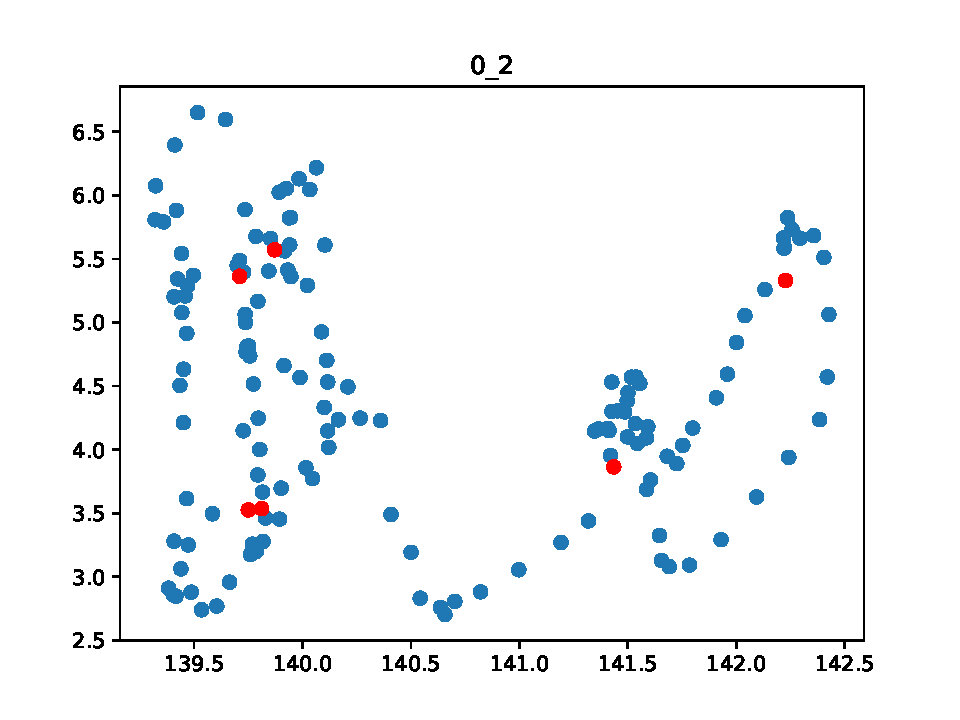
\includegraphics[width=0.45\textwidth]{../plots/0_2.pdf}
    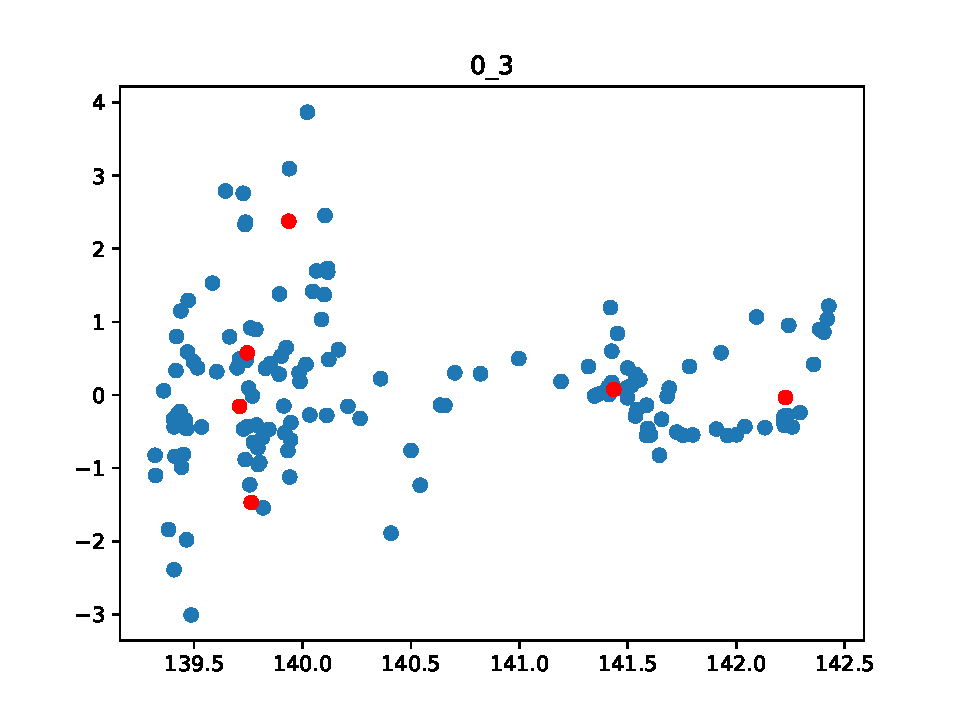
\includegraphics[width=0.45\textwidth]{../plots/0_3.pdf}
    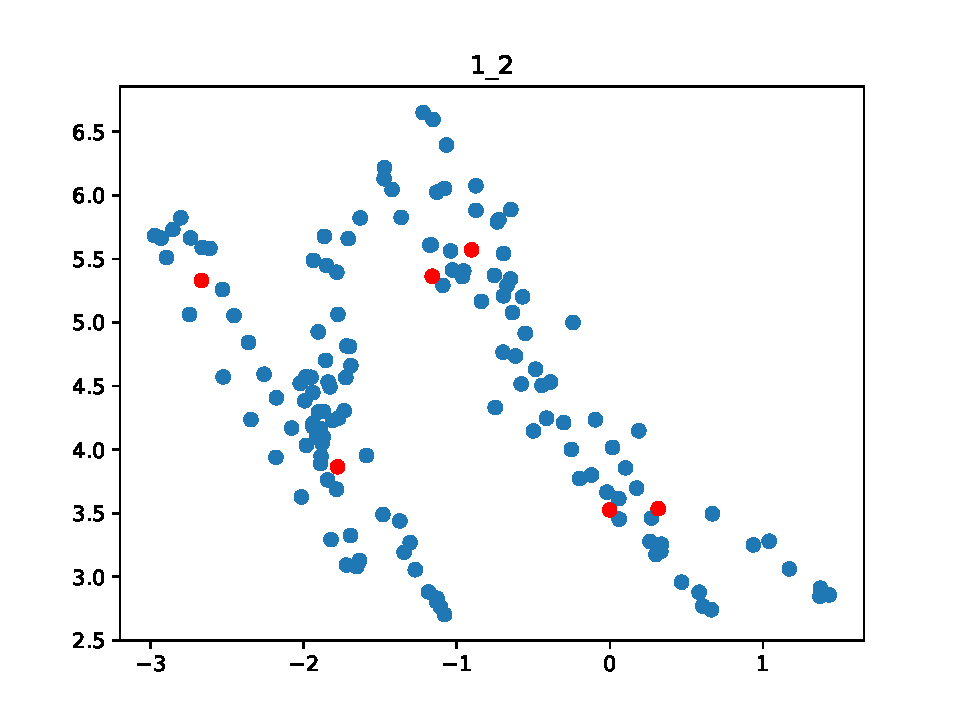
\includegraphics[width=0.45\textwidth]{../plots/1_2.pdf}
    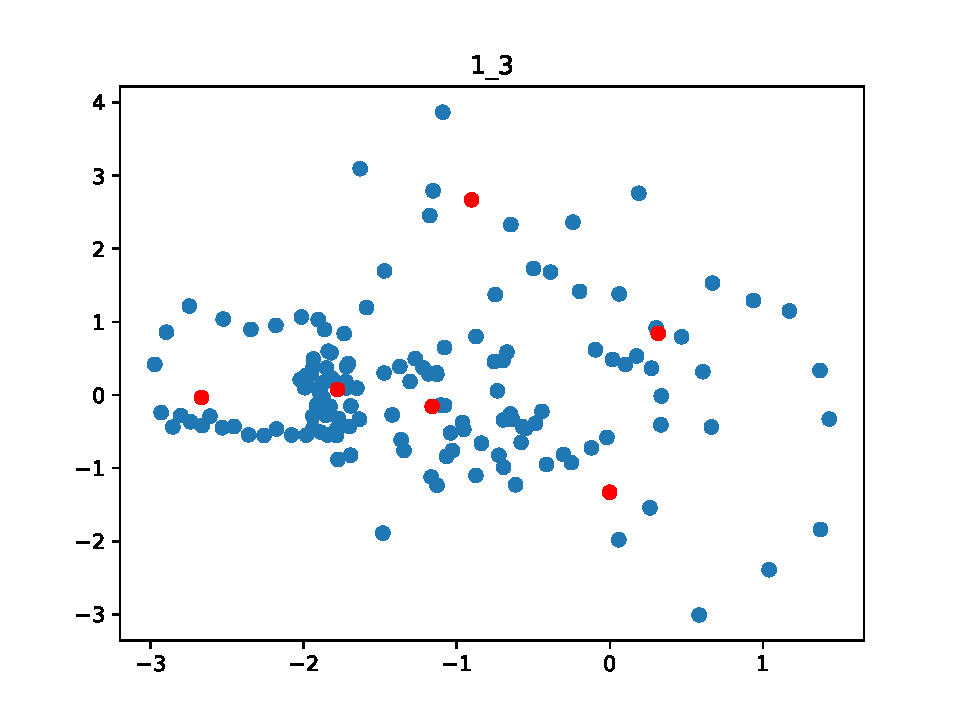
\includegraphics[width=0.45\textwidth]{../plots/1_3.pdf}
    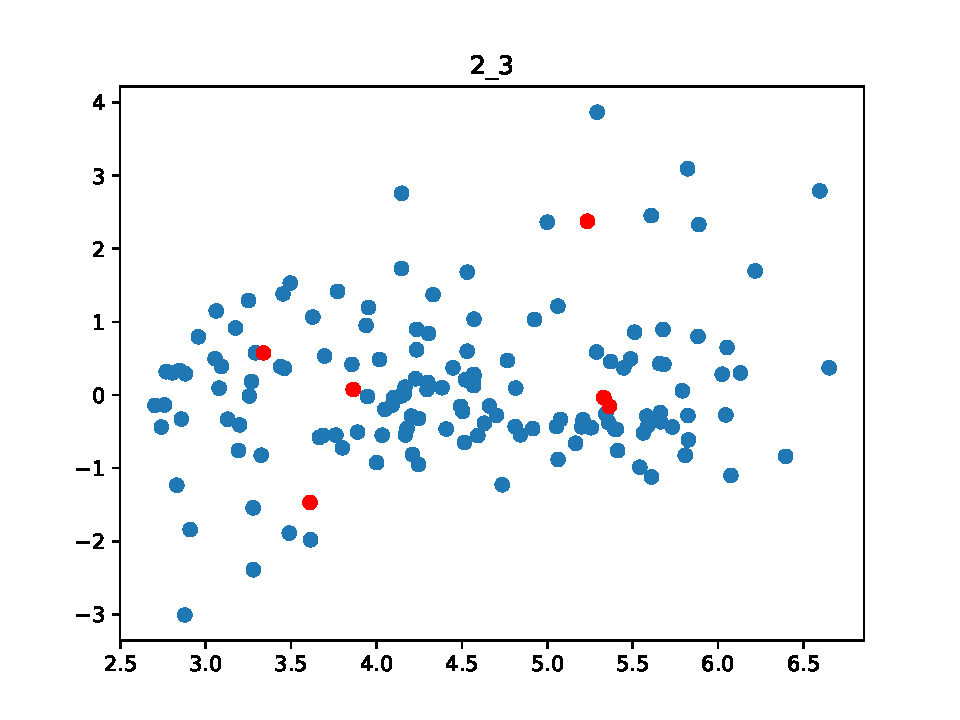
\includegraphics[width=0.45\textwidth]{../plots/2_3.pdf}
    \caption{\label{fig:2dplots} Data (blue) and 6 centroids (red) obtained by the $k$-means algorithm.}
\end{figure}
We can see that the locations of the centroids make sense, especially on some plots.


\end{document}  

